%-------------------------------------------------------------------------------
%-------------------------------------------------------------------------------
%-------------------------------------------------------------------------------
\chapter{Cinétique d'un gaz parfait}
%-------------------------------------------------------------------------------
%-------------------------------------------------------------------------------
%-------------------------------------------------------------------------------
\vskip -2cm

{\sf
La théorie cinétique des gaz vise à expliquer le comportement
macroscopique d'un gaz à partir des mouvements des particules qui le
composent. Depuis la naissance de l'informatique, de nombreuses
simulations numériques ont permis de retrouver les lois de
comportement de différents modèles de gaz comme celui du gaz parfait.
Ce sujet s'intéresse à un gaz parfait monoatomique. 

Nous considérerons
que le gaz étudié est constitué de $N$ particules sphériques, toutes
identiques, de masse $m$ et de rayon $R$, confinées dans un récipient
rigide. Les simulations seront réalisées dans un espace à une, deux ou
trois dimensions ; le récipient contenant le gaz sera, suivant le cas,
un segment de longueur $L$, un carré de côté $L$ ou un cube d'arête $L$.
}
%-------------------------------------------------------------------------------
%-------------------------------------------------------------------------------
\subsubsection{Conventions}
%-------------------------------------------------------------------------------
%-------------------------------------------------------------------------------
\begin{itemize}
    \item Pour répondre à une question il est possible de faire appel aux
fonctions définies dans les questions précédentes.
%-------------------------------------------------------------------------------
    \item Dans tout le sujet on suppose que les bibliothèques \type{math},
\type{numpy} et \type{random} ont été importées grâce aux instructions
\begin{lstlisting}
import math
import random
\end{lstlisting}
%-------------------------------------------------------------------------------
\item Ce sujet utilise une syntaxe raccourcie pour les instructions \type{if} suivie d'une seule instruction courte. L'écriture
%-------------------------------------------------------------------------------
\begin{lstlisting}
    if a < 1:
        return True
\end{lstlisting}
%-------------------------------------------------------------------------------
pourra être écrite sous la forme
%-------------------------------------------------------------------------------
\begin{lstlisting}
    if a < 1: return True
\end{lstlisting}
%-------------------------------------------------------------------------------
\item Ce sujet utilise la syntaxe des annotations pour préciser le types des
arguments et du résultat des fonctions à écrire. Ainsi
%-------------------------------------------------------------------------------
\begin{lstlisting}
def maFonction(n:int, x:float, l:[str]) -> (int, [int]):
\end{lstlisting}
%-------------------------------------------------------------------------------
signifie que la fonction \type{maFonction} prend trois arguments, le
premier est un entier, le deuxième un nombre à virgule flottante et le
troisième une liste de chaînes de caractères et qu'elle renvoie un
couple dont le premier élément est un entier et le deuxième une liste d'entier. 
{\bf Il n'est pas demandé aux candidats de recopier les entêtes avec
annotations telles qu'elles sont fournies dans ce sujet}, ils peuvent
utiliser des entêtes classiques. 
\begin{lstlisting}
def maFonction(n, x, l):
\end{lstlisting}
Les candidats veilleront cependant à décrire
précisément le rôle des fonctions qu'ils définissent.
%-------------------------------------------------------------------------------
\item \type{random.random()} renvoie un nombre flottant tiré aléatoirement
dans $\bigl[0,1\bigr[$ suivant une distribution uniforme
\end{itemize}
%-------------------------------------------------------------------------------
%-------------------------------------------------------------------------------
%-------------------------------------------------------------------------------
\section{Initialisation}
%-------------------------------------------------------------------------------
%-------------------------------------------------------------------------------
%-------------------------------------------------------------------------------
Pour pouvoir réaliser une simulation, il convient de disposer d'une
situation initiale, c'est-à-dire d'un ensemble de particules réparties
dans le récipient et dotées d'une vitesse initiale connue. Cette
partie s'intéresse au positionnement aléatoire d'un ensemble de
particules.
%-------------------------------------------------------------------------------
%-------------------------------------------------------------------------------
\subsection{Placement en dimension 1}
%-------------------------------------------------------------------------------
%-------------------------------------------------------------------------------
Nous cherchons d'abord comment placer $N$ particules (sphères de rayon
$R$) le long d'un segment de longueur $L$ sans qu'elles se chevauchent
ni qu'elles sortent du segment. La figure ci-dessous montre
quelques exemples de placements possibles avec $N=5$, $R=0,5$ et $L=10$.
%--------------------------------------------------------------------------
\begin{center}
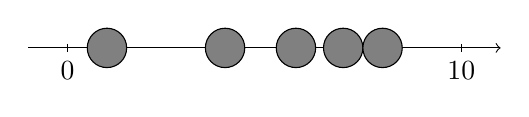
\begin{tikzpicture}[scale=0.5]
\draw[->](-1, 0) -- (11, 0);
\draw (0, 0.1) -- (0, -0.1) node[below] {0};
\draw (10, 0.1) -- (10, -0.1) node[below] {10};
\foreach \x in {1.0, 4.0, 5.8, 7.0, 8.0}
  \draw[fill=gray] (\x, 0) circle (0.5);
\end{tikzpicture} 
\end{center}
%--------------------------------------------------------------------------
\begin{center}
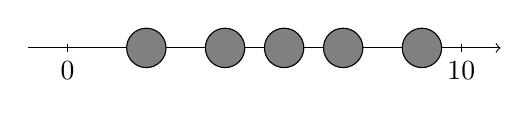
\begin{tikzpicture}[scale=0.5]
\draw[->](-1, 0) -- (11, 0);
\draw (0, 0.1) -- (0, -0.1) node[below] {0};
\draw (10, 0.1) -- (10, -0.1) node[below] {10};
\foreach \x in {2.0, 4.0, 5.5, 7.0, 9.0}
  \draw[fill=gray] (\x, 0) circle (0.5);
\end{tikzpicture} 
\end{center}
%--------------------------------------------------------------------------
\begin{center}
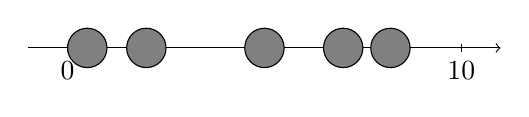
\begin{tikzpicture}[scale=0.5]
\draw[->](-1, 0) -- (11, 0);
\draw (0, 0.1) -- (0, -0.1) node[below] {0};
\draw (10, 0.1) -- (10, -0.1) node[below] {10};
\foreach \x in {0.5, 2.0, 5.0, 7.0, 8.2}
  \draw[fill=gray] (\x, 0) circle (0.5);
\end{tikzpicture} 
\end{center}
%--------------------------------------------------------------------------
\begin{center}
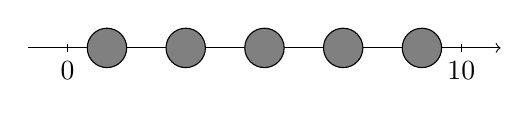
\begin{tikzpicture}[scale=0.5]
\draw[->](-1, 0) -- (11, 0);
\draw (0, 0.1) -- (0, -0.1) node[below] {0};
\draw (10, 0.1) -- (10, -0.1) node[below] {10};
\foreach \x in {1.0, 3.0, 5.0, 7.0, 9.0}
  \draw[fill=gray] (\x, 0) circle (0.5);
\end{tikzpicture} 
\end{center}
%--------------------------------------------------------------------------
La fonction \type{placement1D} construit aléatoirement, à partir des
paramètres géométriques du problème (nombre et rayon des particules,
taille du récipient), une liste de coordonnées correspondant à la
position initiale du centre de chaque particule.
%-------------------------------------------------------------------------------
\begin{lstlisting}[numbers=left]
def placement1D(N:int, R:float, L:float) -> [float]:
    def possible(c:float) -> bool:
        if c < R or c > L - R: return False
        for p in res:
            if abs(c - p) < 2*R: return False
        return True    
    res = []
    while len(res) < N:
        p = L * random.random()
        if possible(p): res.append(p)
    return res
\end{lstlisting}
%-------------------------------------------------------------------------------
%-------------------------------------------------------------------------------
\begin{Exercise}\it 
\begin{enumerate}
    \item Détailler l'action de la ligne 9.
    \item Quelle est la signification du paramètre \type{c} de la
fonction \type{possible} (ligne 2) ?
    \item Expliquer le rôle de la ligne 3.
    \item Expliquer le rôle des lignes 4 et 5.
    \item Donner en une phrase le rôle de la fonction \type{possible}.
 \end{enumerate}
\end{Exercise}
%-------------------------------------------------------------------------------
\begin{Answer}
\begin{enumerate}
    \item À la ligne $9$, on affecte à \type{p} un réel aléatoire entre 0 et $L$.
    \item Le paramètre \type{c} est la position possible d'une particule.
    \item À la ligne 3, on vérifie que la particule est tout entière entre les parois : son centre doit avoir une position entre $R$ et $L-R$.
    \item Les lignes 4 et 5  vérifient que la nouvelle particule n'essaie pas d'occuper une position déjà prise.
    \item \type{possible(c)} teste donc si \type{c} est une position possible pour une nouvelle particule, compte-tenu de celles déjà présentes.
 \end{enumerate}
\end{Answer}
%-------------------------------------------------------------------------------
%-------------------------------------------------------------------------------
\begin{Exercise}[label = {Q:éviter les bords}]\it 
Proposer une nouvelle version de la ligne 9 permettant d'éviter certains rejets de la part de la fonction \type{possible}.
\end{Exercise}
%-------------------------------------------------------------------------------
\begin{Answer} On peut éviter de tester l'inclusion entre les parois en choisissant le centre entre $R$ et $L-R$ :
\begin{lstlisting}
def placement1D(N, R, L):
    
    def possible(c:float) -> bool:
        for p in res:
            if abs(c - p) < 2*R: return False
        return True
    
    res = []
    while len(res) < N:
        p = R + (L - 2*R)*random.random()
        if possible(p): res.append(p)
    return res
\end{lstlisting}
\end{Answer}
%-------------------------------------------------------------------------------
%-------------------------------------------------------------------------------
\begin{minipage}{0.6\textwidth}
\begin{Exercise}[label = {Q:blocage}]\it 
On considère l'appel \type{placement1D(4, 0.5, 5)} et on suppose que les trois premières particules ont été placées aux points d'abscisses 1, 1,5 et 4 (voir ci-contre). 

Quelle sera la suite du déroulement de la fonction \type{placement1D} ?
\end{Exercise}
\end{minipage}
%-------------------------------------------------------------------------------
\begin{minipage}{0.4\textwidth}
\begin{center}
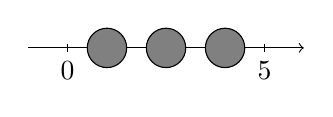
\begin{tikzpicture}[scale=0.5]
\draw[->](-1, 0) -- (6, 0);
\draw (0, 0.1) -- (0, -0.1) node[below] {0};
\draw (5, 0.1) -- (5, -0.1) node[below] {5};
\foreach \x in {1.0, 2.5, 4.0}
  \draw[fill=gray] (\x, 0) circle (0.5);
\end{tikzpicture} 
\end{center}
\end{minipage}
%-------------------------------------------------------------------------------
\begin{Answer}

Avec les trois premières particules placées, il ne reste plus d'espace de largeur $1$ disponible. 

Quel que soit la valeur de $p$, \type{possible(p)} va renvoyer \type{False} et la boucle \type{while} tournera sans fin.
\end{Answer}
%-------------------------------------------------------------------------------
%-------------------------------------------------------------------------------
\begin{Exercise}\it 
Quelle est la complexité temporelle\footnote{On comptera le nombre de comparaisons.}
 de la fonction \type{placement1D} dans le cas\footnote{On admettra que, dans ce cas, la fonction \type{possible(p)} renvoie \type{True} à chaque appel.} où $N \ll N_{\rm max}$, nombre maximal de particules de rayon $R$ pouvant être placées sur un segment de longueur $L$ ?
\end{Exercise}
%-------------------------------------------------------------------------------
\begin{Answer}
On suppose donc que  la boucle \type{while} est effectuée $N$ fois.

À chaque passage on compare la position avec celles des particules déjà placées on fait donc $0 + 1 + 2 + \cdots + (N-1)=\frac{N(N-1)}2$ comparaisons la complexité est un ${\cal O}(N^2)$.
\end{Answer}
%-------------------------------------------------------------------------------
%-------------------------------------------------------------------------------
\begin{Exercise}[label = Q:recommencer]\it 
Pour remédier de manière simple à la situation de la question \ref{Q:blocage}, on décide de recommencer à zéro le placement des particules dès qu'une particule est rejetée par la fonction \type{possible}. 

Réécrire les lignes 7 à 11 de la fonction \type{placement1D} pour mettre en œuvre cette décision.
\end{Exercise}
%-------------------------------------------------------------------------------
\begin{Answer}
\begin{lstlisting}
def placement1D(N, R, L):
    
    def possible(c:float) -> bool:
        for p in res:
            if abs(c - p) < 2*R: return False
        return True
    
    res = []
    while len(res) < N:
        p = R + (L - 2*R)*random.random()
        if possible(p): 
            res.append(p)
        else:
            res = []
    return res
\end{lstlisting}
\end{Answer}
%-------------------------------------------------------------------------------
%-------------------------------------------------------------------------------
\subsection{Optimisation du placement en dimension 1}
%-------------------------------------------------------------------------------
%-------------------------------------------------------------------------------
Pour placer aléatoirement $N$ particules le long d'un segment, nous envisageons une approche plus efficace que celle étudiée dans la partie précédente.

L'idée est de calculer l'espace laissé libre sur le segment cible par $N$ particules\footnote{C'est-à-dire La longueur totale diminuée du diamètre de toutes les particules.}  puis de répartir aléatoirement cet espace libre entre les particules. Afin de conserver une répartition uniforme des particules dans tout le segment, nous utilisons l'algorithme suivant :
\begin{enumerate}
\item déterminer $\ell$, espace laissé libre par les $N$ particules
dans le segment $[0, L[$ ;

\item placer aléatoirement dans le segment $[0, \ell[$, $N$
particules virtuelles ponctuelles ($R=0$) ; 

à cette étape, deux particules peuvent occuper la même abscisse : il n'y a
pas de conflit ;

\item remplacer chaque particule virtuelle par une particule réelle de
rayon $R$ en décalant toutes les particules (réelles et virtuelles)
situées plus à droite de façon à dégager l'espace nécessaire.
\end{enumerate}

\medskip

{\bf Exemple} : $L = 10$, $R = 0.5$, $N = 5$.


On choisit les positions : 
\begin{center}
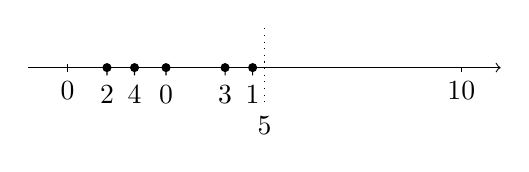
\begin{tikzpicture}[scale=0.5]
\draw[->](-1, 0) -- (11, 0);
\draw (0, 0.1) -- (0, -0.1) node[below] {0};
\draw[dotted] (5, 1) -- (5, -1) node[below] {5};
\draw (10, 0) -- (10, -0.1) node[below] {10};
\foreach \x/\i in {1.0/2, 1.7/4, 2.5/0, 4.0/3, 4.7/1}
  \draw[fill=black] (\x, 0) circle (0.1) -- +(0, -0.2) node[below] {\i};
\end{tikzpicture}
\end{center}

On crée la particule 0 et on déplace les suivantes :
\begin{center}
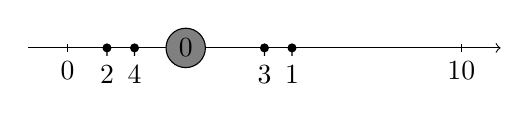
\begin{tikzpicture}[scale=0.5]
\draw[->](-1, 0) -- (11, 0);
\draw (0, 0.1) -- (0, -0.1) node[below] {0};
\draw (10, 0.1) -- (10, -0.1) node[below] {10};
\foreach \x/\i in {3/0}
  {\draw[fill=gray] (\x, 0) circle (0.5);
   \node at (\x, 0) {\i};};
\foreach \x/\i in {1.0/2, 1.7/4, 5.0/3, 5.7/1}
  \draw[fill=black] (\x, 0) circle (0.1) -- +(0, -0.2) node[below] {\i};
\end{tikzpicture}
\end{center}

On crée la particule 1 et on déplace les suivantes :
\begin{center}
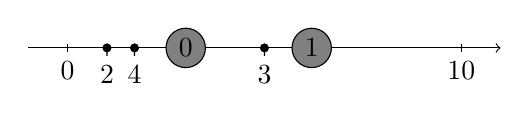
\begin{tikzpicture}[scale=0.5]
\draw[->](-1, 0) -- (11, 0);
\draw (0, 0.1) -- (0, -0.1) node[below] {0};
\draw (10, 0.1) -- (10, -0.1) node[below] {10};
\foreach \x/\i in {3/0, 6.2/1}
  {\draw[fill=gray] (\x, 0) circle (0.5);
   \node at (\x, 0) {\i};};
\foreach \x/\i in {1.0/2, 1.7/4, 5.0/3}
  \draw[fill=black] (\x, 0) circle (0.1) -- +(0, -0.2) node[below] {\i};
\end{tikzpicture}
\end{center}

On crée la particule 2 et on déplace les suivantes :
\begin{center}
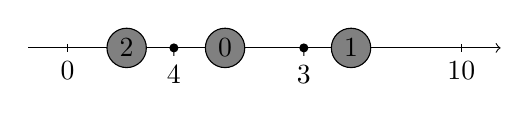
\begin{tikzpicture}[scale=0.5]
\draw[->](-1, 0) -- (11, 0);
\draw (0, 0.1) -- (0, -0.1) node[below] {0};
\draw (10, 0.1) -- (10, -0.1) node[below] {10};
\foreach \x/\i in {1.5/2, 4/0, 7.2/1}
  {\draw[fill=gray] (\x, 0) circle (0.5);
   \node at (\x, 0) {\i};};
\foreach \x/\i in {2.7/4, 6.0/3}
  \draw[fill=black] (\x, 0) circle (0.1) -- +(0, -0.2) node[below] {\i};
\end{tikzpicture}
\end{center}

On crée la particule 3 et on déplace les suivantes :
\begin{center}
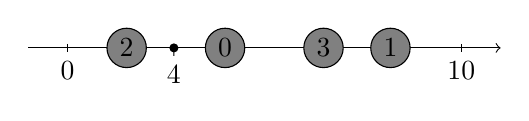
\begin{tikzpicture}[scale=0.5]
\draw[->](-1, 0) -- (11, 0);
\draw (0, 0.1) -- (0, -0.1) node[below] {0};
\draw (10, 0.1) -- (10, -0.1) node[below] {10};
\foreach \x/\i in {1.5/2, 4/0, 6.5/3, 8.2/1}
  {\draw[fill=gray] (\x, 0) circle (0.5);
   \node at (\x, 0) {\i};};
\foreach \x/\i in {2.7/4}
  \draw[fill=black] (\x, 0) circle (0.1) -- +(0, -0.2) node[below] {\i};
\end{tikzpicture}
\end{center}

On crée la particule 4 et on déplace les suivantes :
\begin{center}
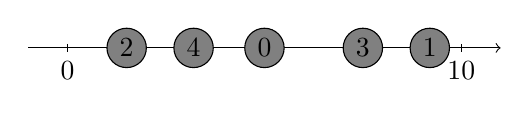
\begin{tikzpicture}[scale=0.5]
\draw[->](-1, 0) -- (11, 0);
\draw (0, 0.1) -- (0, -0.1) node[below] {0};
\draw (10, 0.1) -- (10, -0.1) node[below] {10};
\foreach \x/\i in {1.5/2, 3.2/4, 5/0, 7.5/3, 9.2/1}
  {\draw[fill=gray] (\x, 0) circle (0.5);
   \node at (\x, 0) {\i};};
\end{tikzpicture}
\end{center}
%-------------------------------------------------------------------------------
%-------------------------------------------------------------------------------
\begin{Exercise}\it 
Écrire la fonction \type{placement1Drapide(N, R, L)}
qui implante cet algorithme et renvoie la liste des coordonnées des
centres de \type{N} particules de rayon \type{R} réparties
aléatoirement le long d'un segment situé entre les abscisses $0$ et
\type{L}. 

On précise que l'ordre de la liste résultat n'est pas important.
\end{Exercise}
%-------------------------------------------------------------------------------
\begin{Answer} On doit écarter toutes les boules qui suivent de la valeur d'un diamètre mais aussi écarter d'un rayon la boule actuelle.
\begin{lstlisting}
def placement1Drapide(N, R, L):
    # Etape 1
    l = L - 2*N*R
    # Etape 2
    res=[]
    for i in range(N):
        res.append(l*random.random())
    #Etape 3
    for i in range(N):
        pos=res[i]
        for j in range(N):
            if res[j]>= pos and j !=i :
                res[j] = res[j] + 2*R
        res[i] = res[i] + R
    return res
\end{lstlisting}
\end{Answer}
%-------------------------------------------------------------------------------
%-------------------------------------------------------------------------------
\begin{Exercise}\it 
Quelle est la complexité de la fonction \type{placement1Drapide} ? Commenter.
\end{Exercise}
%-------------------------------------------------------------------------------
\begin{Answer}
Les deux premières étapes se font en temps linéaire en fonction de $N$.

Pour la troisième étape, les deux boucles imbriquées induisent un nombre d'opérations de l'ordre de $N^2$.

On a encore une complexité en ${\cal O}(N^2)$ mais il n'y a plus le risque d'une complexité plus importante en cas densité de particules trop grande.
\end{Answer}
%-------------------------------------------------------------------------------
%-------------------------------------------------------------------------------
\subsection{Utilisation d'un tri}
%-------------------------------------------------------------------------------
%-------------------------------------------------------------------------------
On suppose maintenant qu'entre l'étape 2 et l'étape 3 on effectue le tri des position par ordre croissant par le tri-fusion.

Dans l'exemple illustré ci-dessus, la liste des positions initiales était 
\type{[2.5, 4.7, 1.0, 4.0, 1.7]} et le tri fournit la liste 
\type{[1.0, 1.7, 2.5, 4.0, 4.7]}.

On supposera écrite une fonction \type{tri\_fusion(liste)} qui renvoie une liste qui comporte les mêmes éléments que la liste passée en paramètre mais placé en ordre croissant.

{\bf On ne demande pas d'écrire cette fonction}
%-------------------------------------------------------------------------------
%-------------------------------------------------------------------------------
\begin{Exercise}\it 
Donner rapidement le principe du tri-fusion. On n'expliquera pas la fusion.

Quelle est sa complexité ?
\end{Exercise}
%-------------------------------------------------------------------------------
\begin{Answer}
Le tri fusion sépare la liste en deux partie de tailles quasi-égales, trie récursivement les deux partie puis fusionne les deux listes triées. Ce travail n'est effectué que pour les listes de taille 2 au moins.

Sa complexité est un ${\cal O}\bigl(\log(N)\bigr)$.
\end{Answer}
%-------------------------------------------------------------------------------
%-------------------------------------------------------------------------------
\begin{Exercise}\it 
Écrire la fonction \type{placement1DplusRapide(N, R, L)}
qui implante l'algorithme ci-dessus en insérant le tri et en exploitant le caractère trié de la liste pour effectuer l'étape avec une complexité en ${\cal O}(N)$.

Quelle est maintenant la complexité de la fonction ?
\end{Exercise}
%-------------------------------------------------------------------------------
\begin{Answer}
\begin{lstlisting}
def placement1Drapide(N, R, L):
    # Etape 1
    l = L - 2*N*R
    # Etape 2
    res=[]
    for i in range(N):
        res.append(l*random.random())
    # Tri
    res = tri_fusion(res)
    # Etape 3
    for i in range(N):
        res[i] = res[i] + R + 2*i*R
    return res
\end{lstlisting}

La complexité est celle de la portion la plus lente, c'est un ${\cal O}\bigl(\log(N)\bigr)$.
\end{Answer}
%-------------------------------------------------------------------------------
%-------------------------------------------------------------------------------
\subsection{Dimension quelconque}
%-------------------------------------------------------------------------------
%-------------------------------------------------------------------------------
L'algorithme optimisé pour un segment, n'est pas utilisable pour des espaces de dimensions supérieures. Nous allons donc généraliser la fonction \type{placement1D} pour la transformer en une fonction
utilisable dans un espace de dimension 1, 2 ou 3.
%-------------------------------------------------------------------------------
%-------------------------------------------------------------------------------
\begin{Exercise}\it 
En s'inspirant de la fonction \type{placement1D}, écrire la
fonction d'entête
\begin{lstlisting}
def placement(D:int, N:int, R:float, L:float) -> [[float]]:
\end{lstlisting}
qui renvoie la liste des coordonnées des centres\footnote{Sous forme de listes de $D$ réels.} de \type{N} particules sphériques de rayon \type{R} placées aléatoirement dans un récipient de
côté \type{L} dans un espace à \type{D} dimensions. 

Les modifications prévues aux questions \ref{Q:éviter les bords} et \ref{Q:recommencer} seront prises en compte dans cette fonction.
\end{Exercise}
%-------------------------------------------------------------------------------
\begin{Answer}
On écrit une fonction \type{distance} qui calcule la distance entre deux particules.
\begin{lstlisting}
def distance(p1, p2):
    n = len(p1) # aussi len(p2)
    d = 0
    for i in range(n):
        d = d + (p1[i] - p2[i])**2
    return d**(1/2)
\end{lstlisting}
Il reste à adapter la fonction \type{placement} en créant des particules de bonnes dimensions.
\begin{lstlisting}
def placement(D, N, R, L):
    def possible(c):
        for p in res:
            if distance(c, p) < 2*R: 
                return False
        return True
        
    res=[]
    while len(res) < N:
        p = [0]*D
        for i in range(D):
            p[i] = R + random.random()*(L-2*R)
        if possible(p): 
            res.append(p)
        else:
            res=[]
    return res
\end{lstlisting}
\end{Answer}
%-------------------------------------------------------------------------------
\newpage
%-------------------------------------------------------------------------------
%-------------------------------------------------------------------------------
\section{Exploitation des résultats}
%-------------------------------------------------------------------------------
%-------------------------------------------------------------------------------
%-------------------------------------------------------------------------------
On simule le mouvement de particules en comptant le nombre de chocs sur les parois du contenant. On généralise les calculs en ne supposant plus que les particules sont identiques. Les résultats sont enregistrés dans base de données à trois tables : 
%-------------------------------------------------------------------------------
\[
\tikzstyle{table}=[draw,shape=rectangle,text width=30mm,align=center,minimum height=6mm]
\tikzpicture
\node[table] at (-1,  0.0) {\bf SIMULATION};
\node[table] at (-1, -0.6) (CPSI) {NUM};
\node[table] at (-1, -1.2) {DEB};
\node[table] at (-1, -1.8) {DUR};
\node[table] at (-1, -2.4) {DIM};
\node[table] at (-1, -3.0) {N};
\node[table] at (-1, -3.6) {L};
\node[table] at (4,  0.0) {\bf REBOND};
\node[table] at (4, -0.6) (CSSI) {SI\_NUM};
\node[table] at (4, -1.2) {NUM};
\node[table] at (4, -1.8) (CSPA) {PA\_NUM};
\node[table] at (4, -2.4) {T};
\node[table] at (4, -3.0) {DIR};
\node[table] at (4, -3.6) {VIT};
\node[table] at (4, -4.2) {VP};
\node[table] at (9,  0.0) {\bf PARTICULE};
\node[table] at (9, -0.6) (CPPA) {NUM};
\node[table] at (9, -1.2) {NOM};
\node[table] at (9, -1.8) {M};
\node[table] at (9, -2.4) {R};
\draw[thick, <->] (CPSI) -- +(2.5, 0) |-  (CSSI);
\draw[thick, <->] (CSPA) -- +(2.5, 0) |-  (CPPA);
\endtikzpicture
\]
%--------------------------------------------------------------------------
\subsubsection{SIMULATION}
%--------------------------------------------------------------------------
C'est la table qui donne les caractéristiques de chaque simulation effectuée :
    \begin{itemize}
\item \type{NUM} numéro d'ordre de la simulation (clef primaire),
\item \type{DEB} date et heure du lancement du programme de simulation,
\item \type{DUR} durée (en secondes) de la simulation,
\item \type{DIM} nombre de dimensions de l'espace de simulation,
\item \type{N} nombre de particules pour cette simulation,
\item \type{L} (en mètres) taille du récipient utilisé pour la simulation.
\end{itemize}
%--------------------------------------------------------------------------
\subsubsection{PARTICULE}
%--------------------------------------------------------------------------
C'est la table qui donne les types de particules considérées :
\begin{itemize}
\item \type{NUM} numéro (entier) identifiant le type de particule (clef primaire).
\item \type{NOM} nom de ce type de particule.
\item \type{M} masse de la particule (en grammes).
\item \type{R} rayon (en mètres) de la particule.
\end{itemize}
%--------------------------------------------------------------------------
\subsubsection{REBOND}
%--------------------------------------------------------------------------
Cette table liste les chocs des particules avec les parois du récipient.
\begin{itemize}
\item \type{SI\_NUM} numéro d'ordre de la simulation ayant généré ce rebond.
\item \type{NUM} numéro d'ordre du rebond au sein de cette simulation.
\item \type{PA\_NUM} numéro du type de particule concernée par ce rebond.
\item \type{T} temps de simulation (en secondes) auquel ce rebond est arrivé.
\item \type{DIR} paroi concernée : entier non nul de l'intervalle \type{[-DIM, DIM]} donnant la direction de la normale à la paroi. Ainsi $-1$ désigne la paroi située en $x=0$, $1$ désigne la paroi située en $x=L$ , $-2$ désigne la paroi située en $y=0$. \dots
\item \type{VIT} norme de la vitesse de la particule qui rebondit.
\item \type{VP} valeur absolue de la composante de la vitesse normale à la paroi.
\end{itemize}


\newpage

%-------------------------------------------------------------------------------
%-------------------------------------------------------------------------------
\begin{Exercise}\it 
Proposer une clef primaire pour la table \type{REBOND}, elle comporte plus d'une colonne.
\end{Exercise}
%-------------------------------------------------------------------------------
\begin{Answer}
On doit différentier les rebonds de chaque simulation :

\type{(SI\_NUM, NUM)} est une clef primaire.
\end{Answer}
%-------------------------------------------------------------------------------
%-------------------------------------------------------------------------------
\begin{Exercise}\it 
Écrire une requête SQL qui donne le nom des particules qui ont une masse supérieure à $5.10^{-23}$ grammes (\type{5e-23}).
\end{Exercise}
%-------------------------------------------------------------------------------
\begin{Answer}
\begin{lstlisting}[language=SQL]
select NOM
from PARTICULE
where M > 5e-23
\end{lstlisting}
\end{Answer}
%-------------------------------------------------------------------------------
%-------------------------------------------------------------------------------
\begin{Exercise}\it 
Écrire une requête SQL qui donne, pour chaque simulation, le nombre  (\type{count}) de rebonds enregistrés et la vitesse moyenne (\type{avg}) des particules qui frappent une paroi.
\end{Exercise}
%-------------------------------------------------------------------------------
\begin{Answer}
\begin{lstlisting}[language=SQL]
select SI_NUM, count(), avg(VIT)
from REBOND
group by SI_NUM
\end{lstlisting}
\end{Answer}
%-------------------------------------------------------------------------------
%-------------------------------------------------------------------------------
\begin{Exercise}\it 
Quelles sont les noms des particules qui sont intervenues dans la simulation de numéro 1472 ?
\end{Exercise}
%-------------------------------------------------------------------------------
\begin{Answer}
\begin{lstlisting}[language=SQL]
select distinct p.NOM
from REBOND as r join PARTICULE as p on r.PA_NUM = p.NUM
where r.SI_NUM = 1472
\end{lstlisting}
\end{Answer}
%-------------------------------------------------------------------------------
%-------------------------------------------------------------------------------
\begin{Exercise}\it 
Quelles sont les durées des simulation qui ont simulé plus de 100\,000 rebonds ?
\end{Exercise}
%-------------------------------------------------------------------------------
\begin{Answer}
\begin{lstlisting}[language=SQL]
select r.SI_NUM, count() as nb, s.DUR
from REBOND as r join SIMULATION as s
group by r.SI_NUM
having nb > 1e5
\end{lstlisting}
\end{Answer}
%-------------------------------------------------------------------------------
%-------------------------------------------------------------------------------
\begin{Exercise}\it 
Écrire une requête SQL qui, pour la simulation de numéro $4782$, calcule, pour chaque paroi, la variation de quantité de mouvement due aux chocs des particules sur cette paroi tout au long de la simulation (\type{sum}). 

On se rappellera que lors du rebond d'une particule sur une paroi la composante de sa vitesse normale à la paroi est inversée, ce qui correspond à une variation de quantité de mouvement de $2m\|v_\perp\|$ où $m$ désigne la masse de la particule et $v_\perp$ la composante de sa vitesse normale à la paroi.
\end{Exercise}
%-------------------------------------------------------------------------------
\begin{Answer}
\begin{lstlisting}[language=SQL]
select r.DIR, sum(2*p.M*r.VP)
from REBOND as r join PARTICULE as p on  r.PA_NUM = p.NUM
WHERE SI_NUM = 4782
group by DIR
\end{lstlisting}
\end{Answer}
%-------------------------------------------------------------------------------
%-------------------------------------------------------------------------------

